% \chapter{Von der Theorie $\theoryBSO$ zu einem Interpretationsansatz}
%\chapter{Grundideen des Interpretationsansatzes}\label{chap:bso-grundideen}
\chapter{Grundlagen der \strukt}\label{chap:bso-grundideen}

    In diesem Kapitel wird dargestellt, wie ich von der in Kapitel~\ref{chap:bs} eingeführten Theorie der ordinären Entitäten des Brentanoraumes zur \strukt, einer Interpretation für $\theoryBSO$, komme.

    In den Abschnitten \ref{sec:raumreg} bis \ref{sec:zusammenfassung} greife ich die dort eingeführten Ideen auf. In diesem Kapitel stehen jedoch die Vorstellungen, die meinen Interpretationsansätzen zugrunde liegen, im Mittelpunkt. Redundanzen lassen sich hierbei nicht vermeiden und werden der Abgeschlossenheit der Darstellung zuliebe in Kauf genommen.

    In den Abschnitten \ref{sec:universum} und \ref{sec:prim-rel-1} wird die \strukt eingeführt.
    Für eine exakte Ausformulierung der darin verwendeten Begriffe werden etablierte Werkzeuge aus der Topologie und weitere topologische Definitionen benötigt, die in den folgenden Kapiteln bereitgestellt werden.
    Deshalb beschränke ich mich erst einmal auf die Darstellung der grundlegenden Ideen.
    Auch für eigentlich mathematische Begriffe wie \glqq Dimension\grqq\ verlasse ich mich hier auf das intuitive Verständnis des Lesers.

    Die Lücken des vorgestellten Ansatzes werden in Abschnitt \ref{sec:ausblick} zusammengefasst und deren Lösungen in Ausblick gestellt.

    \section{Raumregionen}\label{sec:raumreg}
        Ich betrachte den Raum --~hier auch als einbettender Raum bezeichnet~-- als homogenen, unendlich ausgedehnten unveränderlichen Rahmen, in dem sich physikalische Prozesse abspielen.
        Dies steht im Widerspruch zu der in [\cite{baumann-r-2016-53-a}] vertretenen Vorstellung, dass der Raum von materiellen Objekten, die ihn einnehmen, generiert wird.
%         Dies steht möglicherweise im Widerspruch zu den Weltbild der Autoren der $\theoryBS$-Theorie,
%         die davon ausgehen, dass der Raum von materiellen Objekten, die ihn einnehmen, generiert wird.
        Für das Ziel der Arbeit, einen Ansatz für einen konstruktiven Konsistenzbeweis für $\theoryBS$ vorzustellen, sind diese Unterschiede, soweit ich es absehen kann, jedoch nicht relevant.

        Teilmengen des einbettenden Raumes, die von materiellen Körpern eingenommen werden können, heißen Raumregionen.
        \marginpar{Raumregionen und Topoide}
        Da materielle Körper endlich sind, müssen sie beschränkt sein, nicht jedoch notwendigerweise zusammenhängend, wie im vorherigen Kapitel ausgeführt wurde. 
        Zusammenhängende Raumregionen%
        \footnote{
            genauer gesagt $2$-dimensional zusammenhängende
        }
        heißen Topoide.
	
        Im Gegensatz zu materiellen Körpern können sich Raumregionen gegenseitig durchdringen,
        da jede \textit{mögliche} Teilmenge des einbettenden Raumes, die von materiellen Körpern eingenommen werden \textit{kann}, als Raumregion bezeichnet wird.
        
        Des Weiteren werden Raumregionen hier als echt $3$-dimensional angenommen. 
        Wir gehen also davon aus, dass materielle Körper überall eine nicht zu vernachlässigende Ausdehnung haben.
        \marginpar{Raumregionen sind echt $3$-dimensional}
        Dies ist physikalisch gesehen wohl sinnvoll. 
        Dennoch kann man darüber nachdenken, inwieweit diese Annahme geeignet ist, materielle Körper im fraglichen Größenordnungsbereich zu beschreiben, anstatt auf dieser Granularitätsebene bestimmte Körper als niederdimensional zu betrachten (siehe Abbildung \ref{fig:echt-3-dim}).
        Zu beachten ist außerdem, dass Raumregionen durchaus Stellen haben können, an denen sie niederdimensional zusammenhängen, wie im vorherigen Kapitel beschrieben wurde.
	
        \begin{figure}[ht]
            \centering
            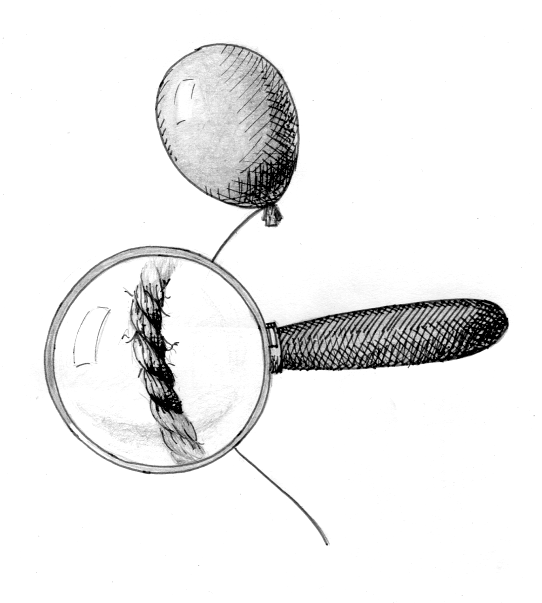
\includegraphics[height=7cm]{luise/echt-3-dim.png}
            \caption{Materielle Körper sind überall echt $3$-dimensional}
            \label{fig:echt-3-dim}
        \end{figure}

        Wie im vorherigen Kapitel werde ich auch hier nicht strikt zwischen Raumregionen und den Objekten, die bestimmte Raumregionen einnehmen, unterscheiden. Mit \glqq Erde\grqq\ ist dann die Raumregion gemeint, die von der Erde eingenommen wird. Analoges gilt für Begriffe wie \glqq Erdoberfläche\grqq , \glqq Küstenlinie\grqq\ u.s.w., die sich auf niederdimensionale Objekte beziehen.
        Niederdimensional heißt im Folgenden immer $0$-, $1$- oder $2$-dimensional.
	
    \section{Niederdimensionale Raumentitäten}\label{sec:niederdimensionale-re}
        Eine Flächenregion ist eine $2$-dimensionale Teilmenge der Oberfläche einer Raumregion -- beispielsweise die obere Seite eines Würfels. 
        \marginpar{Flächenregion,\\Koinzidenz}
        Berühren sich zwei Raumregionen an einer Fläche, so hat jede ihre eigene Flächenregion als Grenze. Nehmen wir beispielsweise zwei aufeinander liegende Würfel, so berühren sich die obere Seite des unteren Würfels und die untere Seite des oberen Würfels, sie werden jedoch nicht als gleich betrachtet. Wir sagen, die beiden Seiten koinzidieren.
        
        Damit wir Flächenregionen als gleich betrachten, müssen sie nicht notwendigerweise die gleichen Raumregionen begrenzen. 
        \marginpar{Gleichheit von Flächenregionen}
        Es genügt, wenn die Raumregionen von denen sie erzeugt werden \glqq von der gleichen Seite kommen\grqq .
        Nehmen wir beispielsweise die Landfläche der Antarktis. Wir könnten sie als Teil der Erdoberfläche sehen oder als Teil der Oberfläche der Antarktischen Platte. In beiden Fällen kommen die erzeugenden Raumregionen \glqq von unten\grqq . Somit sind die beiden Flächenregionen gleich.
    
        Koinzidenz ist eine Äquivalenzrelation auf den niederdimensionalen Raumentitäten, d.h. insbesondere, dass eine Flächenregion immer mit sich selbst koinzidiert. 
        \marginpar{euklidische Fläche}
        Die Äquivalenzklassen der Koinzidenz auf den Flächenregionen werde ich im Weiteren \glqq euklidische Flächen\grqq\ nennen. 
        Während eine euklidische Fläche lediglich durch die Punkte charakterisiert wird, die sie im einbettenden Raum einnimmt, \glqq weiß\grqq\ die Flächenregion, von welcher Seite die Raumregion kommt, die durch sie begrenzt wird.

        Welche Teilmengen des einbettenden Raumes als euklidische Flächen gelten, hängt unter anderem davon ab, welche Mengen als Raumregionen zugelassen sind. Insbesondere wollen wir sicherstellen, dass die gesamte Oberfläche einer beliebigen Raumregion eine Flächenregion ist. Daraus ergibt sich als weitere Bedingung, dass Raumregionen überall einen $2$-dimensionalen Rand haben sollen. Dies verbietet insbesondere niederdimensionale Löcher in Raumregionen. Die Erde ohne ihren Mittelpunkt beispielsweise wäre keine Raumregion, da bei diesem Körper der Mittelpunkt ein Randpunkt wäre und die Oberfläche somit an dieser Stelle $0$-dimensional.
    
        Zwei Flächenregionen überlappen, wenn ihre euklidischen Flächen gemeinsame $2$-dimensionale Teile haben und diese gemeinsamen Teile wiederum Teile haben, die Raumregionen begrenzen, die von der gleichen Seite kommen (siehe Abbildung \ref{fig:overlap}).
        \marginpar{Überlappung}
    
%         \todo[inline]{Bilder zu overlap zusammenfassen}
%         
        \begin{figure}[ht]
            \centering
            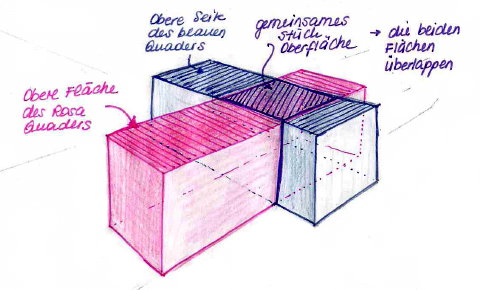
\includegraphics[height=5cm]{luise/overlap.png}
            \caption{Zwei Flächen, die überlappen}
            \label{fig:overlap}
        \end{figure}
        
        \begin{figure}[ht]
            \centering
            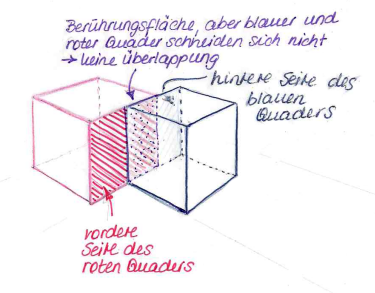
\includegraphics[height=5cm]{luise/no-overlap.png}
            \caption{Zwei Flächen, die koinzidierende Teile haben, aber nicht überlappen}
            \label{fig:no-overlap}
        \end{figure}

    %\subsubsection{Von Flächenregionen zu Linienregionen}
        Analog zur Konstruktion von Flächenregionen und euklidischen Flächen aus Raumregionen können wir aus Flächenregionen Linienregionen und euklidische Linien erzeugen. 
        \marginpar{Linienregion,\\euklidische Linie}
        Eine Linienregion ist eine $1$-dimensionale Teilmenge des Randes einer Flächenregion und eine euklidische Linie ist die Menge der Punkte im einbettenden Raum, die dieser Linienregion entspricht und dabei die dahinter liegenden Raum- und Flächenregionen vergisst.
        Ob zwei Linienregionen gleich sind oder lediglich koinzidieren hängt nun von den zugrundeliegenden Flächenregionen ab und diese wiederum von den dahinter liegenden Raumregionen.

    %\subsubsection{Von Linienregionen zu Punktregionen}
        Auf gleiche Weise entstehen Punktregionen und euklidische Punktmengen aus Linienregionen. 
        \marginpar{Punktregion,\\euklidische Punktmenge}
        Zwei Punktregionen können nur gleich sein, wenn die Linienregionen, durch die sie erzeugt werden, ein gewisses Stück weit gleich aussehen, also überlappen.

        Raumregionen, euklidische Flächen, Linien und Punktmengen werden euklidische Entitäten genannt.
        \marginpar{(niederdimensionale) euklidische Entität}
        Die letzten drei heißen niederdimensionale euklidische Entitäten.

    %\section{Eigenschaften ordinärer Raumentitäten (Zusammenfassung)}\label{sec:zusammenfassung}
    \section{Eigenschaften ordinärer Raumentitäten}\label{sec:zusammenfassung}
        Der hier vorgestellte Interpretationsansatz baut auf den Eigenschaften der ordinären Raumentitäten auf, die ich im Folgenden deshalb zusammenfasse.

        \paragraph{Eigenschaften von Raumregionen:} 
        \begin{itemize}
            \item[(R0)] Raumregionen sind beschränkt.
            \item[(R1)] Sie sind überall echt $3$-dimensional, insbesondere enthalten sie keine niederdimensionalen Ausläufer.
            \item[(R2)] Ihr Rand ist überall echt $2$-dimensional.
            \item[(R3)] Sie enthalten keine niederdimensionalen Löcher.
        \end{itemize}
        
        \paragraph{Eigenschaften von euklidischen Flächen:} 
        \begin{itemize}
            \item[(F0)] Euklidische Flächen liegen auf dem Rand von Raumregionen.
            \item[(F1)] Sie sind überall echt $2$-dimensional, insbesondere enthalten sie keine $1$- oder $0$-dimensionalen Ausläufer oder $3$-dimensionalen Klumpen.
            \item[(F2)] Ihr Rand ist überall echt $1$-dimensional.
            \item[(F3)] Sie enthalten sie keine $1$- oder $0$-dimensionalen Löcher.
        \end{itemize}
            
        \paragraph{Eigenschaften von Flächenregionen:}
        \begin{itemize}
            \item[(F4)] Flächenregionen begrenzen Raumregionen.
            \item[(F5)] Zu jeder Flächenregion gehört genau
%\todo[inline]{\small FL-Absicherung 03.05.: ``genau'' i.O.? Analog für nachfolgende *-regionen ... -> BH: i.O.}
                        eine euklidische Fläche.
            \item[(F6)] Eine Flächenregion ist die ihr zugehörige euklidische Fläche, zusammen mit der Information, welche Raumregionen durch sie begrenzt werden.
            \item[(F7)] Verschiedene Raumregionen, die durch die gleiche Flächenregion begrenzt werden, kommen an jedem Punkt der zugehörigen euklidischen Fläche aus derselben Richtung.
        \end{itemize}

        \paragraph{Eigenschaften von euklidischen Linien:} 
        \begin{itemize}%[Eigenschaften von Linien]
            \item[(L0)] Euklidische Linien liegen auf dem Rand von euklidischen Flächen.
            \item[(L1)] Sie sind überall echt $1$-dimensional, insbesondere enthalten sie keine isolierten Punkte.
            \item[(L2)] Ihr Rand ist überall echt $0$-dimensional.
            \item[(L3)] Sie enthalten sie keine $0$-dimensionalen Löcher.
        \end{itemize}
            
        \paragraph{Eigenschaften von Linienregionen:}
        \begin{itemize}
            \item[(F4)] Linienregionen begrenzen Flächenregionen.
            \item[(F5)] Zu jeder Linienregion gehört genau eine euklidische Linie.
            \item[(F6)] Eine Linienregion ist die ihr zugehörige euklidische Linie, zusammen mit der Information, welche Flächenregionen durch sie begrenzt werden.
            \item[(F7)] Verschiedene Flächenregionen, die durch die gleiche Linienregion begrenzt werden, kommen an jedem Punkt der zugehörigen euklidischen Fläche aus derselben Richtung.
        \end{itemize}
            
        \paragraph{Eigenschaften von euklidischen Punktmengen:} 
        \begin{itemize}%[Eigenschaften von Punktmengen]
            \item[(P0)] Euklidische Punktmengen liegen auf dem Rand von euklidischen Linien.
        \end{itemize}
        
        \paragraph{Eigenschaften von Punktregionen:}
        \begin{itemize}
            \item[(F4)] Punktregionen begrenzen Linienregionen.
            \item[(F5)] Zu jeder Punktregion gehört genau eine euklidische Punktmenge.
            \item[(F6)] Eine Punktregion ist die ihr zugehörige euklidische Punktmenge, zusammen mit der Information welche Linienregionen durch sie begrenzt werden.
            \item[(F7)] Verschiedene Linienregionen, die durch die gleiche Punktregion begrenzt werden, kommen an jedem Punkt der zugehörigen euklidischen Punktmenge aus derselben Richtung.
        \end{itemize}

% 	
% 	\paragraph{Gleichheit von ordinären Raumentitäten} 
% 	\begin{itemize}%[Gleichheit von ordinären Raumentitäten]
% 		\item[(G3)] Zwei Raumregionen sind gleich, wenn sie die gleichen Punkte des einbettenden Raumes einnehmen.
% 		\item[(G2)] Zwei Flächenregionen sind gleich, wenn ihre zugehörigen euklidischen Flächen gleich sind und die Raumregionen, die durch sie begrenzt werden überall von der gleichen Seite kommen.
% 		\item[(G1)] Zwei Linienregionen sind gleich, wenn ihre zugehörigen euklidischen Linien gleich sind und \textcolor{red}{sie eine Umgebung haben, in der die Grenzflächen, die durch sie begrenzt werden, gleich aussehen}.
% 		\item[(G0)] Zwei Grenzpunktmengen sind gleich, wenn sie die gleichen Punkte im umgebenden Raum einnehmen und die Grenzlinien, durch die sie erzeugt werden gemeinsame Stücke haben in der Nähe der Punkte.
% 	\end{itemize}
% 	
% 	\paragraph{Koinzidenz} 
% 	\begin{itemize}
% 	    \item[(K0)] Zwei Punktregionen koinzidieren, wenn ihre zugehörigen euklidischen Punktmengen gleich sind.
%         \item[(K1)] Zwei Linienregionen koinzidieren, wenn ihre zugehörigen euklidischen Linien gleich sind.
%         \item[(K2)] Zwei Flächenregionen koinzidieren, wenn ihre zugehörigen euklidischen Flächen gleich sind.
% 		\item[(K3)] Zwei Raumregionen können nicht koinzidieren.
% 	\end{itemize}

	\paragraph{Koinzidenz} 
	\begin{itemize}
	    \item[(K0)] Zwei niederdimensionale Raumentitäten koinzidieren, wenn die ihnen zugehörigen euklidischen Entitäten gleich sind.
	\end{itemize}

	
%\subsection{Repräsentanten und Objektäquivalenz}
    \section{Das Universum der \strukt}\label{sec:universum}

        Eine Flächenregion begrenzt unendlich viele Raumregionen.
        Kennen wir jedoch eine Raumregion, die von einer bestimmten Flächenregion $u$ begrenzt wird, so wissen wir, dass jede andere Raumregion, die an jedem Punkt der zugehörigen euklidischen Fläche von der gleichen Seite kommt, auch von $u$ begrenzt wird.
        Raumregionen hingegen, für die das nicht der Fall ist, werden nicht von $u$ begrenzt (siehe Abbildung \ref{fig:sb}).
%         Betrachte als Beispiel Abbildung \ref{fig:sb}. 
%         Dort gilt:
%         Wenn $x$ durch $u$ begrenzt wird, dann auch $y$, nicht jedoch $z$.

        \begin{figure}[ht]
            \centering
            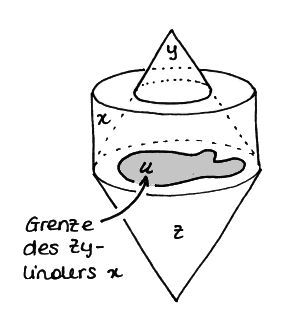
\includegraphics[height=7cm]{abb/sb.png}
            \caption[Räumliche Grenzen]{Räumliche Grenzen: Wenn die Flächenregion $u$ die Raumregion $x$ begrenzt, so auch die $y$, nicht jedoch $z$}
            \label{fig:sb}
        \end{figure}

        Um eine Flächenregion zu kennen, genügt es also, die ihr zugehörige euklidische Fläche und eine Raumregion zu kennen, die von ihr begrenzt wird.
        Jedes Paar $(A,B)$ aus einer Raumregion $A$ und einer euklidischen Fläche $B$ auf dem Rand von $A$ repräsentiert also eine Flächenregion.

        Ähnlich, aber komplizierter, verhält es sich bei Linienregionen. 
        Um eine Linienregion zu kennen, müssen wir die ihr zugehörige euklidische Linie und eine Flächenregion kennen, die von ihr begrenzt wird. 
        Da Flächenregionen durch Paare repräsentiert werden, braucht es also Tripel, um Linienregionen zu repräsentieren.
        Zwei Linienregionen zu den gleichen euklidischen Linien und Flächen, die durch die Tripel $(A_1, B, C)$ und $(A_2, B, C)$ repräsentiert werden, können verschieden sein, wenn $A_1$ und $A_2$ von verschiedenen Seiten auf $B$ zukommen. 
        Eine ähnliche Situation ist in Abbildung \ref{fig:objektaeq-linien} dargestellt (Beispiel 1).

        \begin{figure}[ht]
            \centering
            \includegraphics[height=5cm]{abb/objektaeq-linien.png}
            \caption{Beispiele für äquivalente (2) und nicht äquivalente (1) Linienregionen}
            \label{fig:objektaeq-linien}
        \end{figure}
        
        Auf dieser Idee -- dass niederdimensionale Raumentitäten durch Tupel repräsentiert werden -- beruht die \strukt, wobei das Symbol $\rep$ für \glqq repräsentantenbasiert\grqq\ steht.
        Zusammengefasst werden in der folgenden Definition Flächen-, Linien- und Punktrepräsentanten definiert und in Abbildung \ref{fig:repr} verdeutlicht.

        \begin{dfn}[Repräsentanten]\ \vspace{0pt}
            \begin{enumerate}
                \item Ein \spacedlowsmallcaps{Flächenrepräsentant} ist ein Paar $(A,B)$, 
                    bestehend aus einer Raumregion $A$ und einer euklidischen Fläche $B$ auf deren Rand.\\
                    Die \spacedlowsmallcaps{Menge der Flächenrepräsentanten} bezeichnen wir mit $\rep^2$.
                \item Ein \spacedlowsmallcaps{Linienrepräsentant} ist ein Tripel $(A,B,C)$, 
                    wobei $(A,B)$ ein Flächenrepräsentant ist und $C$ eine euklidische Linie auf dem Rand von $B$.\\
                    Die \spacedlowsmallcaps{Menge der Linienrepräsentanten} bezeichnen wir mit $\rep^1$.
                \item Ein \spacedlowsmallcaps{Punktrepräsentant} ist ein Quadrupel $(A,B,C,D)$, 
                    wobei $(A,B,C)$ ein Linienrepräsentant ist und $D$ eine euklidische Punktmenge auf dem Rand von $B$.\\
                    Die \spacedlowsmallcaps{Menge der Punktrepräsentanten} bezeichnen wir mit $\rep^0$.
            \end{enumerate}
        \end{dfn}

        \begin{figure}[ht]
            \centering
            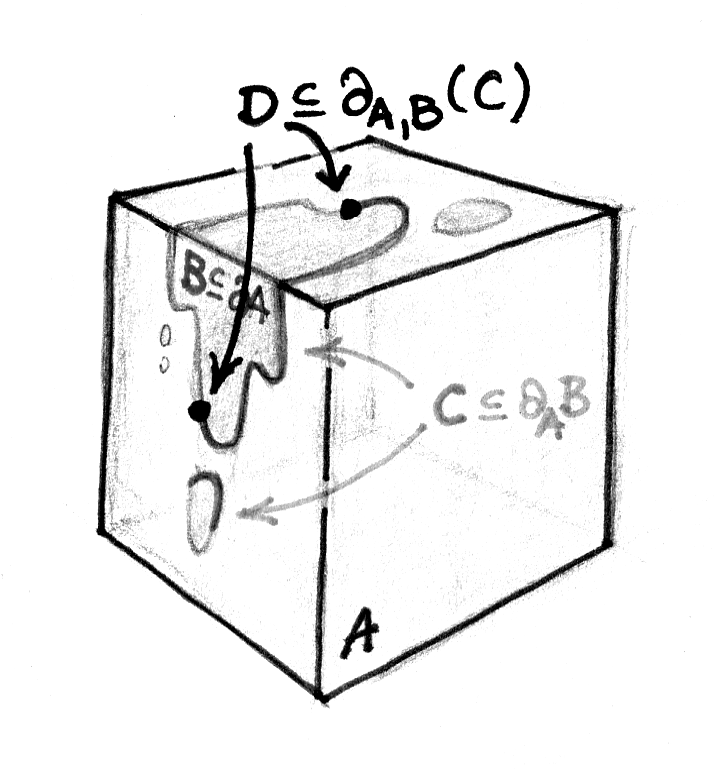
\includegraphics[height=5cm]{luise/repr.png}
            \caption[Grundbegriffe der $\mathcal{R}$-Struktur]{Grundbegriffe der \strukt:\\
                    $A$ ist eine Raumregion, $B$ eine euklidische Fläche, $C$ eine euklidische Linie und $D$ eine euklidische Punktmenge. $(A,B)$ ist ein Flächenrepräsentant, $(A,B,C)$ ein Linienrepräsentant und $(A,B,C,D)$ ein Punktrepräsentant.}
            \label{fig:repr}
        \end{figure}

        Eine Äquivalenzrelation auf der Menge der Repräsentanten, für die zwei Repräsentanten äquivalent sind, wenn sie die gleiche Raumentität repräsentieren, heißt Objektäquivalenz.
        \marginpar{Objektäquivalenz}
        Eine Objektäquivalenz erfasst also in geeigneter Weise, was es heißt, dass zwei Raumentitäten \glqq von der gleichen Seite\grqq\ oder \glqq aus der gleichen Richtung\grqq\ kommen.
        Niederdimensionale Raumentitäten lassen sich also als Äquivalenzklassen einer Objektäquivalenz auffassen, was in folgender Definition präzisiert wird.

        \begin{dfn}[Flächen-, Linien- und Punktregionen]\ \vspace{8pt}

            \noindent
            Sei $\sim$ eine Objektäquivalenz.
            %
            \begin{enumerate}
        %			
                \item Für $(A,B) \in \rep^2$ bezeichnet 
                    \begin{align*}
                        [A,B] := \{(A',B') \in \rep^2 \mid (A',B') \sim (A,B)\}
                    \end{align*}
                    die Äquivalenzklasse von $(A,B)$ bezüglich der Objektäquivalenz.\\
                    Diese Äquivalenzklassen heißen \spacedlowsmallcaps{Flächenregionen}.
                    
                \item Für $(A,B,C) \in \rep^1$ bezeichnet
                    \begin{align*}
                        [A,B,C] := \{(A',B',C') \in \rep^1 \mid (A',B',C') \sim (A,B,C)\}
                    \end{align*}			 
                    die Äquivalenzklasse von $(A,B,C)$ bezüglich der Objektäquivalenz.\\
                    Diese Äquivalenzklassen heißen \spacedlowsmallcaps{Linienregionen}.
        %			
                \item Für $(A,B,C,D) \in \rep^0$ bezeichnet
                    \begin{align*}
                        &[A,B,C,D] := \\
                        &\{(A',B',C',D') \in \rep^0 \mid (A',B',C',D') \sim (A,B,C,D)\}
                    \end{align*}			 
                    die Äquivalenzklasse von $(A,B,C,D)$ bezüglich der Objektäquivalenz.\\
                    Diese Äquivalenzklassen heißen \spacedlowsmallcaps{Punktregionen}.
        %			
            \end{enumerate}
            %
            \noindent	
                Für $i \in \{0,1,2\}$ ist $\univ^i := \rep^i /_\sim$ die \spacedlowsmallcaps{Menge der Äquivalenzklassen} von $\rep^i$.\\
                $\univ^3$ ist die \spacedlowsmallcaps{Menge der Raumregionen}.
                
        \end{dfn}
        
        In Abbildung \ref{fig:objektaeq-flaechen} sind Beispiele für äquivalente und nicht äquivaleten Flächenregionen dargestellt.
        %
        \begin{figure}[ht]
            \centering
            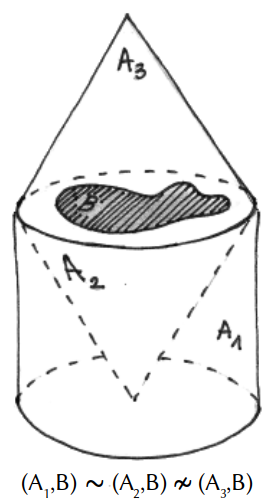
\includegraphics[height=7cm]{gfx/objektaeq-flaechen.png}
            \caption{Beispiele für äquivalente und nicht äquivalente Flächenrepräsentanten}
            \label{fig:objektaeq-flaechen}
        \end{figure}

        Damit können wir das Universum der \strukt definieren, das aus den Raum-, Flächen-, Linien- und Punktregionen besteht.

        \begin{dfn}[Universum]\ \vspace{8pt}

            \noindent
            Das Universum der \strukt ist definiert als
            \begin{align*}
                \univ = \univ^3 \cup \univ^2 \cup \univ^1 \cup \univ^0
            \end{align*}
                    
        \end{dfn}
        
        Da $\univ^3$, $\univ^2$, $\univ^1$ und $\univ^0$ paarweise disjunkt sind, lässt sich die folgende Funktion auf $U$ definieren:
    
        \begin{dfn}[Dimensionsfunktion]\ \\
            $\Gdim : \univ \to \N$ ist definiert durch
            $$ \Gdim(x) = i \quad \Leftrightarrow \quad x \in \univ^i $$
        \end{dfn}



    \section{Primitive Relationen}\label{sec:prim-rel-1}

        Die Interpretation der primitiven Relationen in $\theoryBSO$ unter der \strukt kann vollständig auf die gewählte Objektäquivalenz zurückgeführt werden, die im Folgenden mit $\sim$ bezeichnet wird.
        %Zur Unterscheidung werden die Symbole der Struktur mit einem hochgestellten $\strukt$ versehen.

        Die Interpretation des Symbols $\GSReg$ als Menge der Raumregionen ist selbsterklärend.
        \marginpar{$\GSReg$}

        Für die Interpretation des Symbols $\Gsb$ rufen wir uns ins Gedächtnis:
        Eine Flächenregion, die durch einen Flächenrepräsentanten $(A_1,B)$ repräsentiert wird, begrenzt eine Raumregion $A_2$, wenn $A_1$ und $A_2$ überall auf der gleichen Seite von $B$ liegen. In diesem Fall sind dann $(A_1,B)$ und $(A_2, B)$ äquivalent.
        Diese Überlegung lässt sich auf andere Dimensionen erweitern und führt zu folgender Definition:

        \begin{dfn}[Die $\Gsb$-Relation in der \strukt]\ \vspace{0pt}

            \begin{enumerate}
                \item Für $(A_1,B_1) \in \rep^2$, $A_2 \in \univ^3$ gilt 
                    \begin{align*}
                        \Gsb([A_1,B_1],A_2) \quad \Leftrightarrow \quad (A_1,B_1) \sim (A_2,B_1)
                    \end{align*}
                \item Für $(A_1,B_1,C_1) \in \rep^1$, $(A_2,B_2) \in \rep^2$ gilt 
                    \begin{align*}
                        &\Gsb([A_1,B_1,C_1],[A_2,B_2]) \quad \\
                        &\Leftrightarrow  \quad (A_1,B_1,C_1) \sim (A_2,B_2,C_1)
                    \end{align*}
                \item Für $(A_1,B_1,C_1,D_1) \in \rep^0$, $(A_2,B_2,C_2) \in \rep^1$ gilt 
                    \begin{align*}
                        &\Gsb([A_1,B_1,C_1,D_1],[A_2,B_2,C_2]) \quad \\
                        &\Leftrightarrow  \quad (A_1,B_1,C_1,D_1) \sim (A_2,B_2,C_2,D_1)
                    \end{align*}
                %\item Für $x \in \U^i$, $y \in \U^j$ mit $i+1 \neq j$ gilt $\neg sb(x,y)$
                \item Für $x, y$ mit $\Gdim(x) + 1 \neq \Gdim(y)$ gilt $\neg \Gsb(x,y)$
            \end{enumerate}
            
        \end{dfn}
        
        Als direkte Folgerung aus dieser Definition ergibt sich folgender Satz
        
        \begin{satz}\label{satz:sb-einfacher-fall}\ \vspace{0pt}
            
            \begin{itemize}
                \item Für alle Flächenrepräsentanten $(A,B) \in \rep^2$ gilt: \\$\Gsb([A,B],A)$
                \item Für alle Linienrepräsentanten $(A,B,C) \in \rep^1$ gilt: \\$\Gsb([A,B,C],[A,B])$
                \item Für alle Punktrepräsentanten $(A,B,C,D) \in \rep^0$ gilt: \\$\Gsb([A,B,C,D],[A,B,C])$
            \end{itemize}
        \end{satz}
    
        Zwei niederdimensionale Raumentitäten koinzidieren, wenn die ihnen zugehörigen euklidischen Entitäten gleich sind. Damit ergibt sich als Interpretation für das $\Gscoinc$-Symbol:
    
        \begin{dfn}[Die $\Gscoinc$-Relation in der \strukt]\ \vspace{0pt}

            \begin{enumerate}
                \item Für $A_1, A_2 \in \univ^3$ gilt: $\neg \Gscoinc(A_1,A_2)$
                \item Für $(A_1,B_1), (A_2,B_2) \in \rep^2$ gilt 
                    \begin{align*}
                        \Gscoinc([A_1,B_1],[A_2,B_2]) \quad \Leftrightarrow  \quad B_1 = B_2
                    \end{align*}
                \item Für $(A_1,B_1,C_1), (A_2,B_2,C_2) \in \rep^1$ gilt 
                    \begin{align*}
                        \Gscoinc([A_1,B_1,C_1],[A_2,B_2,C_2]) \quad \Leftrightarrow  \quad C_1 = C_2
                    \end{align*}
                \item Für $(A_1,B_1,C_1,D_1), (A_2,B_2,C_2,D_2) \in \rep^0$ gilt 
                    \begin{align*}
                        &\Gscoinc([A_1,B_1,C_1,D_1],[A_2,B_2,C_2,D_2]) \\
                        &\Leftrightarrow  \quad D_1 = D_2
                    \end{align*}
                %\item Für $x \in \U^i$, $y \in \U^j$ mit $i \neq j$ gilt $\neg scoinc(x,y)$
                \item Für $x, y$ mit $\Gdim(x) \neq \Gdim(y)$ gilt $\neg \Gscoinc(x,y)$.
            \end{enumerate}
            
        \end{dfn}%
%        
        Aus dieser Definition ergibt sich trivialerweise:
        
        \begin{satz}\ \\
            Die $\Gscoinc$-Relation ist eine Äquivalenzrelation auf $\univ^2 \cup \univ^1 \cup \univ^0$.
        \end{satz}
    
        Die Überlegungen zur Interpretation des Symbols $\Gspart$ ähneln den Überlegungen zur Interpretation von $\Gsb$.
    
        Für Raumregionen ist klar: Eine Raumregion ist räumlicher Teil einer anderen, wenn sie eine Teilmenge dieser ist.
    
        Damit eine Flächenregion räumlicher Teil einer anderen ist, muss die ihr zugehörige euklidische Fläche Teil der euklidischen Fläche der anderen sein.
        Dies reicht jedoch nicht, wie Abbildung \ref{fig:spart-flaechen} zeigt.
        
        Seien $(A_1,B_1)$ und $(A_2,B_2)$ Flächenrepräsentanten mit $B_1 \subseteq B_2$. Damit $[A_1,B_1]$ räumlicher Teil von $[A_2,B_2]$ ist, müssen $A_1$ und $A_2$ von der gleichen Seite auf $B_1$ zukommen. Dann ist $(A_1,B_2)$ äquivalent zu $(A_2, B_1)$.
            
        Analoge Bedingungen gelten für die $\Gspart$-Beziehung von Linienregionen. Beispiele hierzu sind in Abbildung \ref{fig:spart-linien} dargestellt.
        Nun können wir definieren:

        \begin{dfn}[Die $\Gspart$-Relation in der \strukt]\ \vspace{0pt}

            \begin{enumerate}
                \item Für $A_1, A_2 \in \univ^3$ gilt $\Gspart(A_1,A_2)$ gdw.\ $A_1 \subseteq A_2$
        %		
                \item Für $(A_1,B_1), (A_2,B_2) \in \rep^2$ gilt \\
                $\Gspart([A_1,B_1],[A_2,B_2])$ gdw.\ 
                    \begin{enumerate}
                        \item $B_1 \subseteq B_2$
                        \item $(A_1, B_1) \sim (A_2, B_1)$
                    \end{enumerate}	
        %			
                \item Für $(A_1,B_1,C_1), (A_2,B_2,C_2) \in \rep^1$ gilt \\
                $\Gspart([A_1,B_1,C_1],[A_2,B_2,C_2])$ gdw.\ 
                    \begin{enumerate}
                        \item $C_1 \subseteq C_2$
                        \item $(A_1, B_1, C_1) \sim (A_2, B_2, C_1)$
                    \end{enumerate}	
        %			
                \item Für $(A_1,B_1,C_1,D_1), (A_2,B_2,C_2,D_2) \in \rep^0$ gilt \\
                $\Gspart([A_1,B_1,C_1,D_1],[A_2,B_2,C_2,D_2])$ gdw.\
                    \begin{enumerate}
                        \item $D_1 = D_2$
                        \item $(A_1, B_1, C_1, D_1) \sim (A_2, B_2, C_2, D_1)$
                    \end{enumerate}	
        %			
                \item Für $x, y$ mit $\Gdim(x) \neq \Gdim(y)$ gilt $\neg \Gspart(x,y)$
        %		
            \end{enumerate}
            
        \end{dfn}
        
        
    
        \begin{figure}[ht]
            \centering
            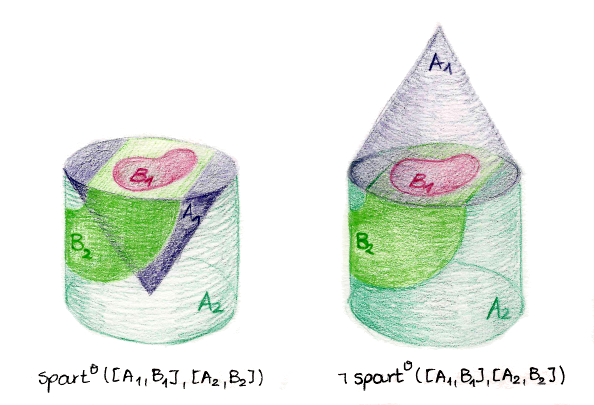
\includegraphics[height=7cm]{abb/spart-flaechen.png}
            \caption{Beispiel und Gegenbeispiel zu $\Gspart$ bei Flächenregionen}
            \label{fig:spart-flaechen}
        \end{figure}

        \begin{figure}[ht]
            \centering
            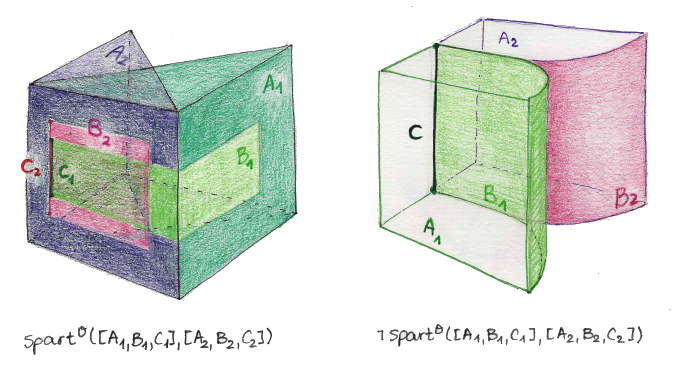
\includegraphics[width=0.9\textwidth]{abb/spart-linien.png}
            \caption{Beispiel und Gegenbeispiel zu $\Gspart$ bei Linienregionen}
            \label{fig:spart-linien}
        \end{figure}

    \section{Ausblick}\label{sec:ausblick}
        Der hier skizzierte Interpretationsansatz ist bislang unvollständig.

        Zum einen ist offen, in welchem Raum die euklidischen Entitäten zu finden sind ($\R^3$ als Vektorraum, affiner Raum, ... ).
        In dieser Arbeit habe ich mich für den $\R^3$ als mit der euklidischen Metrik ausgestatten metrischen Raum entschieden. 
        Dieser wird in Kapitel \ref{chap:topologie-grundlagen} eingeführt.

        Welche Teilmengen dieses Raumes die gewünschten Eigenschaften von euklidischen Entitäten aufweisen, ist eine anspruchsvolle Frage, die im Rahmen dieser Arbeit nicht erschöpfend untersucht werden kann.
        Ich nutze hier die einfachen Mengen, die in Kapitel \ref{chap:topologie-erweiterung} eingeführt werden.
        Sie schließen einige offensichtlich unerwünschte Fälle aus.

        Zu dieser Frage gehört auch, was als Rand der euklidischen Entitäten zählt, auf dem dann die nächst-niedriger-dimensionalen Entitäten zu finden sind.
        Dafür wird ebenfalls in Kapitel \ref{chap:topologie-erweiterung} der sogenannte äußere Rand eingeführt.

        Schließlich muss noch eine Objektäquivalenz definiert werden, die in geeigneter Weise erfasst, was es heißt, wenn zwei Raumentitäten \glqq von der gleichen Seite\grqq\ auf eine dritte zukommen.
        Mit ihrer Einführung in Kapitel \ref{chap:bso-struktur} werden die letzten Lücken in der Definition der \strukt geschlossen.
